% Chapter 3: Literature Review
% Text, tables and figure taken word for word from the survey paper
% "Survey: Optimizing Large Language Models for Low-Latency Inference under
% Resource Constraints" (M. Lootah and S. G. Khawaja), with its own 50 references.

\chapter{Literature Review}
\label{Chapter3}

\section{Introduction}
\label{sec:lr-intro}

Large Language Models (LLMs) have become a major direction in modern artificial intelligence due to their strong performance in language understanding, text generation, reasoning, summarization, and code-related tasks. Their success is mainly driven by transformer-based architectures, which allow models to learn complex contextual relationships from large-scale data. However, the same architectural growth that improves model capability also increases computational cost, memory usage, and inference latency. As a result, deploying LLMs in practical environments remains challenging, especially when the target system has limited hardware resources or strict response-time requirements \cite{survey2021transformers,survey2021ondevice}.

The deployment challenge becomes more significant in low-latency and resource-constrained environments such as edge devices, embedded platforms, mobile systems, and private enterprise servers. In these settings, large models often require high memory bandwidth, powerful GPUs, and considerable energy consumption, which may not always be available. Therefore, efficient LLM deployment requires optimization techniques that reduce model size and inference cost while maintaining acceptable model accuracy. This has motivated increasing research interest in quantization, pruning, sparsity, knowledge distillation, and hybrid compression strategies \cite{frantar2023sparsegpt,ma2023llmpruner,sanh2020distilbert,jiao2020tinybert}.

Quantization is one of the most widely studied approaches for improving LLM efficiency. It reduces the numerical precision of model weights and activations, allowing models to consume less memory and execute faster on supported hardware. Early and influential methods such as LLM.int8(), ZeroQuant, GPTQ, and SmoothQuant demonstrated that post-training quantization can significantly reduce inference cost while preserving model quality \cite{dettmers2022llmint8,yao2022zeroquant,frantar2023gptq,xiao2023smoothquant}. More recent methods, including AWQ, OmniQuant, SpQR, SqueezeLLM, and QuIP, further improve low-bit and weight-only quantization by addressing activation sensitivity, outlier effects, and dense-sparse compression \cite{lin2024awq,dettmers2024spqr,shao2024omniquant,kim2024squeezellm,chee2023quip}.

In addition to quantization, pruning-based compression has also been explored to reduce unnecessary parameters, layers, or structures within LLMs. Methods such as SparseGPT, Wanda, LLM-Pruner, SliceGPT, and ShortGPT show that large models often contain redundancy that can be removed with limited accuracy loss when pruning is carefully designed \cite{frantar2023sparsegpt,ma2023llmpruner,sun2024wanda,ashkboos2024slicegpt,men2024shortgpt}. Other recent works combine pruning with quantization or use mixed-precision strategies to better balance compression ratio, latency reduction, and model performance \cite{xu2026daypq,cho2025sub4bit,wang2025ofqllm}.

Despite these advances, efficient LLM deployment remains an open research problem. Many techniques report strong compression or accuracy results, but their real-world effectiveness depends heavily on hardware support, memory access patterns, batch size, sequence length, and inference framework implementation. In addition, reducing bit-width or removing model structures can introduce accuracy degradation, instability, or limited generalization across different model families. These issues highlight the need for clearer comparisons between compression ratio, latency, energy efficiency, memory usage, and model quality.

This survey reviews recent quantization and compression techniques for low-latency LLM deployment. It focuses on model-level and algorithm-level optimization methods, including post-training quantization, weight-only quantization, activation-aware quantization, mixed-precision quantization, pruning, sparsity, knowledge distillation, and hybrid compression. The main objective is to summarize current progress, compare important techniques, and identify research gaps related to accuracy preservation, hardware-aware evaluation, latency benchmarking, and practical deployment on real-world platforms. Building on these gaps, the survey further proposes a compression framework that coordinates pruning and quantization in a single adaptive pipeline.

The remainder of this survey is organized as follows. Section~\ref{sec:lr-method} describes the survey methodology, including the literature sources, search terms, and inclusion and exclusion criteria used to select the reviewed papers. Section~\ref{sec:lr-review} presents the literature review and comparative analysis, which is divided into five thematic subsections covering quantization-based optimization, pruning and sparsity-based compression, hybrid quantization and pruning, knowledge distillation, and KV-cache compression, with each subsection accompanied by a structured comparison table. Section~\ref{sec:lr-discussion} discusses the comparative findings across these technique families, addressing their prevalence, ease of implementation, latency and model-size benefits, hardware dependencies, and unresolved challenges. Section~\ref{sec:lr-gaps} identifies the main research gaps that remain in the field, and Section~\ref{sec:lr-future} proposes promising future research directions. Section~\ref{sec:lr-proposed} presents a proposed compression framework that builds on the identified gaps and directions, describing its design objectives, pipeline stages, sensitivity-profiling methods, constraint handling, and evaluation strategy. Finally, Section~\ref{sec:lr-conclusion} concludes the survey by summarizing its scope, main findings, and the principal challenges that motivate continued research.

\section{Survey Methodology}
\label{sec:lr-method}

This survey followed a structured literature review approach to identify and analyze recent research on quantization and compression techniques for low-latency LLMs deployment. The literature search was conducted using major academic databases and search platforms, including IEEE Xplore, Google Scholar, ScienceDirect, and relevant survey papers. These sources were selected because they provide access to peer-reviewed journal articles, conference papers, preprints, and recent surveys related to efficient deep learning and LLM optimization.

The search focused on papers published from 2020 onward to ensure that the reviewed work reflects recent developments in LLM compression and deployment. The main search terms included combinations of keywords such as ``large language model quantization,'' ``LLM compression,'' ``low-latency LLM deployment,'' ``post-training quantization,'' ``weight-only quantization,'' ``activation-aware quantization,'' ``mixed-precision quantization,'' ``LLM pruning,'' and ``efficient LLM inference.''

The inclusion criteria were based on publication year, relevance to the survey topic, technical contribution, and experimental validation. Papers were included if they focused on quantization, pruning, sparsity, model compression, or efficient inference for LLMs or transformer-based models. Priority was given to studies that provided experimental results, compared their methods with existing baselines, reported performance metrics such as accuracy, latency, memory reduction, compression ratio, or inference speed, and appeared in reputable journals, conferences, or widely cited preprint repositories.

Papers were excluded if they were published before 2020, were not directly related to quantization or compression, focused only on general deep learning without relevance to LLM deployment, lacked experimental evaluation, or did not provide enough technical detail for comparison. Duplicate papers, non-technical articles, and works with limited relevance to low-latency or resource-constrained deployment were also removed from consideration.

In total, approximately 50 papers were reviewed. These papers were analyzed to identify common optimization techniques, compare their advantages and limitations, and extract research gaps related to efficient, low-latency LLM deployment.

\section{Literature Review and Comparative Analysis}
\label{sec:lr-review}

This section reviews recent research on quantization and compression techniques for low-latency LLM deployment and it is organized according to the main optimization directions found in the reviewed papers, namely quantization-based optimization, pruning and sparsity, hybrid quantization and pruning, knowledge distillation, and KV-cache compression. Each group is analyzed in terms of the problem addressed, methodology, experimental focus, key results, hardware dependencies if mentioned, and remaining research gaps. To make the comparison systematic, every subsection concludes with a structured comparison table.

\emph{Standard hardware} means normal CPUs and GPUs that run regular dense matrix operations. These systems do not need special support. Methods such as structural pruning, layer removal, and knowledge distillation create smaller dense models, so they can usually run faster on standard hardware. \emph{Sparse kernels} are special computation methods that skip weights with zero values. These are important for unstructured pruning because removing individual weights does not automatically make the model faster. Without sparse-kernel support, unstructured pruning may reduce the number of parameters, but it may not reduce inference latency. This support is still limited on many common hardware platforms. \emph{Low-rank execution} means using compressed weight matrices directly as smaller matrix operations instead of rebuilding the original full matrix. Low-rank methods only reduce computation if the inference system can run these factorized matrices efficiently.

\subsection{Quantization-Based Optimization}

Quantization is one of the most common methods used to reduce the cost of running LLMs. In normal training and inference, model weights and activations are usually stored using high-precision formats such as FP16 or FP32. These formats require a large amount of memory and computation. Quantization reduces this cost by representing values using lower precision, such as INT8, INT4, or even lower bit-widths. This can reduce memory usage and improve inference speed, especially when the hardware supports low-bit computation.

LLM.int8() showed how large transformer models can be executed using 8-bit matrix multiplication while maintaining good accuracy \cite{dettmers2022llmint8}. The main problem addressed by this method is that simple 8-bit quantization can damage model quality because LLMs contain sensitive outlier values. To solve this, the method keeps important outlier features in higher precision while quantizing the rest of the computation. This makes the model smaller and faster while reducing accuracy loss, cutting inference memory by roughly half and supporting models up to 175B parameters. However, the method mainly focuses on INT8 quantization and does not fully solve the challenges of more aggressive quantization such as INT4 or 2-bit precision.

ZeroQuant also focuses on post-training quantization for large transformer models \cite{yao2022zeroquant}. Post-training quantization is useful because it does not require retraining the full model, which can be expensive. ZeroQuant makes large models smaller by quantizing their values and training the compressed model to imitate the larger model layer by layer, helping it keep good accuracy. Beyond the algorithm, it provides an optimized inference backend and reports speedups of up to 5.19$\times$ over baseline execution. This method is useful for practical deployment because it reduces the cost of optimization. However, its performance depends on calibration data and may vary depending on the model and hardware used.

GPTQ focuses mainly on weight-only quantization, where the model weights are compressed to lower precision while activations are kept in higher precision \cite{frantar2023gptq}. GPTQ uses approximate second-order information to decide how to quantize weights with less accuracy loss. The method showed that large models can be compressed to 3-bit and 4-bit precision with acceptable degradation, quantizing a 175B-parameter model in about four GPU hours and achieving roughly 3.25$\times$ inference speedup on an A100 GPU. However, because GPTQ mainly quantizes weights, it may not fully reduce activation memory or all runtime costs during inference.

SmoothQuant addresses another important problem in LLM quantization: activation outliers \cite{xiao2023smoothquant}. Activations in LLMs can contain very large values, which makes activation quantization difficult. SmoothQuant solves this by shifting some of the quantization difficulty from activations to weights through an equivalent smoothing transformation, enabling training-free W8A8 quantization with close to FP16 accuracy and around 2$\times$ memory reduction. The method is important because activation quantization can help reduce inference cost further. However, it still depends on calibration data and optimized hardware support.

AWQ, or Activation-aware Weight Quantization, improves low-bit weight quantization by identifying which weights are most important for model performance \cite{lin2024awq}. Instead of treating all weights equally, AWQ protects important weights using activation information and quantizes the rest, enabling INT3 and INT4 weight-only deployment without backpropagation or heavy retraining. AWQ is practical for 4-bit LLM deployment and is widely relevant to low-latency inference. However, it mainly focuses on weight compression and does not fully solve activation or KV-cache memory bottlenecks.

A second group of methods targets near-lossless and learnable post-training quantization. SpQR isolates outlier weights and stores them in higher precision while quantizing the remaining dense weights, achieving relative perplexity loss below one percent and allowing a 33B-parameter model to run on a single 24GB GPU \cite{dettmers2024spqr}. SqueezeLLM attacks the memory-bandwidth bottleneck of generative decoding using dense-and-sparse, sensitivity-aware non-uniform quantization, reaching 3-bit precision while improving quality over earlier methods \cite{kim2024squeezellm}. OmniQuant replaces hand-chosen quantization parameters with learnable weight clipping and learnable equivalent transformations, supporting a wide range of settings from W6A6 down to W2A16 \cite{shao2024omniquant}. These works show that careful outlier handling and calibration can preserve accuracy at low bit-widths, although their runtime gains still depend on optimized kernels.

A third group addresses activation quantization through reordering and rotation. RPTQ reorders activation channels and quantizes them in clusters, pushing activations toward 3-bit precision \cite{yuan2023rptq}. QuaRot applies Hadamard-style rotations that preserve the model function while removing outliers, enabling end-to-end 4-bit inference for weights, activations, and KV cache with about 99 percent zero-shot performance retention on LLaMA2-70B \cite{ashkboos2024quarot}. SpinQuant extends this idea by learning the rotation matrices rather than relying only on random rotations, further reducing outlier-driven error \cite{liu2025spinquant}. These methods are important because activation quantization is required for real latency and memory benefits beyond weight-only compression.

A fourth group pursues extreme and codebook-based compression. QuIP showed that quantization improves when weights and Hessian directions are made incoherent before rounding, providing the first viable 2-bit post-training quantization route with theoretical support \cite{chee2023quip}. QuIP\# builds on this with randomized Hadamard transforms and lattice codebooks for compression at or below 4 bits \cite{tseng2024quipsharp}, while AQLM adapts additive multi-codebook quantization to reach 2 to 3 bits per parameter \cite{egiazarian2024aqlm}. QTIP replaces vector codebooks with trellis-coded quantization to obtain a high effective quantization dimension without exponentially large codebooks \cite{tseng2024qtip}. Pushing precision further, BiLLM and PB-LLM binarize most weights while protecting salient ones \cite{huang2024billm,shang2023pbllm}, and PT-BitNet scales 1.58-bit ternary models through post-training quantization, reporting memory compression between 5.72$\times$ and 6.28$\times$\cite{survey2025ptbitnet}. These methods maximize model-size reduction but carry higher accuracy risk and depend strongly on specialized kernels.

Finally, several works connect quantization to training and deployment. EfficientQAT makes quantization-aware training feasible for large models, producing a 2-bit LLaMA-2-70B model with less than a three-point accuracy drop \cite{chen2025efficientqat}, and PV-Tuning provides a representation-agnostic fine-tuning framework for recovering accuracy after extreme 1 to 2-bit compression \cite{malinovskii2024pvtuning}. ABQ-LLM closes the gap between low-bit algorithms and actual GPU acceleration by supporting arbitrary bit-width combinations with distribution correction \cite{zeng2025abqllm}, and FRM-PTQ preserves internal feature relationships to improve low-bit post-training quantization quality for both weights and activations \cite{survey2026frmptq}. Table~\ref{tab:lr-quant} summarizes and compares these quantization techniques.

\begin{table}[htbp]
\centering
\scriptsize
\caption{Comparison of quantization-based optimization techniques.}
\label{tab:lr-quant}
\renewcommand{\arraystretch}{1.2}
\begin{tabular}{p{\dimexpr 0.186\linewidth-2\tabcolsep\relax}p{\dimexpr 0.307\linewidth-2\tabcolsep\relax}p{\dimexpr 0.307\linewidth-2\tabcolsep\relax}p{\dimexpr 0.200\linewidth-2\tabcolsep\relax}}
\hline
\textbf{Technique [Ref]} & \textbf{Approach / Contribution} & \textbf{Key Reported Results} & \textbf{Hardware \& Complexity} \\
\hline
LLM.int8() \cite{dettmers2022llmint8} & Mixed-precision INT8; keeps outliers in FP16 & $\sim$50\% memory cut; supports up to 175B & Moderate HW; low \\
ZeroQuant \cite{yao2022zeroquant} & PTQ with layer-wise distillation and backend & Up to 5.19$\times$ speedup; $\sim$3$\times$ memory cut & Needs backend; moderate \\
GPTQ \cite{frantar2023gptq} & One-shot weight-only PTQ (second-order) & 3--4-bit; $\sim$3.25$\times$ speedup on A100 & Low-bit kernels; low \\
SmoothQuant \cite{xiao2023smoothquant} & Activation-to-weight smoothing & W8A8; $\sim$2$\times$ memory; 1.56$\times$ speedup & INT8 kernels; low \\
AWQ \cite{lin2024awq} & Activation-aware salient-weight scaling & INT3/INT4 weight-only; accuracy preserved & Low-bit kernels; low \\
SpQR \cite{dettmers2024spqr} & Sparse-quantized outlier isolation & 3--4-bit; $>$4$\times$ cut; $<$1\% perplexity loss & Sparse kernels; moderate \\
OmniQuant \cite{shao2024omniquant} & Learnable clipping and transform for PTQ & W6A6 to W2A16; 70B calibrated in $\leq$16 h & Kernel-dependent; moderate \\
SqueezeLLM \cite{kim2024squeezellm} & Dense-and-sparse non-uniform quantization & Up to 3-bit; up to 2.3$\times$ speedup & Sparse kernels; moderate \\
RPTQ \cite{yuan2023rptq} & Reorder-based activation quantization & 3-bit activations; $\sim$80\% memory cut & HW-dependent; moderate \\
QuaRot \cite{ashkboos2024quarot} & Hadamard rotation removes outliers & W4A4; $\sim$99\% zero-shot retention & Rotated kernels; mod.--high \\
SpinQuant \cite{liu2025spinquant} & Learned rotations for weights, act., KV & 4-bit; $\sim$2.9-point zero-shot gap & Rotated kernels; high \\
QuIP \cite{chee2023quip} & Incoherence processing for 2-bit PTQ & First viable 2-bit weight quantization & Low-bit kernels; moderate \\
QuIP\# \cite{tseng2024quipsharp} & Hadamard incoherence and lattice codebooks & $\leq$4-bit; strong extreme compression & Codebook kernels; high \\
AQLM \cite{egiazarian2024aqlm} & Additive multi-codebook quantization & 2--3 bits per parameter; Pareto-strong & Impl.-dependent; high \\
QTIP \cite{tseng2024qtip} & Trellis-coded quantization and incoherence & State-of-the-art sub-4-bit quality/speed & Trellis kernels; high \\
BiLLM \cite{huang2024billm} & 1-bit PTQ with salient-weight protection & $\sim$1.08-bit; 7B binarized in $\sim$0.5 h & Binary kernels; high \\
PB-LLM \cite{shang2023pbllm} & Partial binarization, salient weights kept & Most weights 1-bit; beats naive binarization & Mixed kernels; high \\
PT-BitNet \cite{survey2025ptbitnet} & Post-training 1.58-bit ternary scaling & 5.7--6.3$\times$ memory cut; latency halved & Ternary kernels; high \\
EfficientQAT \cite{chen2025efficientqat} & Efficient quantization-aware training & 2-bit 70B in 41 h; $<$3-point accuracy drop & Post-QAT kernels; high \\
PV-Tuning \cite{malinovskii2024pvtuning} & Post-compression fine-tuning (1--2-bit) & Pareto-optimal 2-bit LLaMA-2 results & Pairs with codebooks; high \\
ABQ-LLM \cite{zeng2025abqllm} & Arbitrary-bit PTQ with GPU framework & W2A8; 1.6$\times$ accel., 2.7$\times$ memory cut & GPU framework; mod.--high \\
FRM-PTQ \cite{survey2026frmptq} & Feature-relationship matching for low-bit PTQ & W4A4/W3A3; $\sim$2$\times$ throughput gain & Low-bit kernels; moderate \\
\hline
\end{tabular}
\end{table}

\subsection{Pruning and Sparsity-Based Compression}

Pruning aims to remove less important weights, neurons, channels, layers, or structures from a model. Unlike quantization, which changes numerical precision, pruning reduces the number of active parameters or computations. This can theoretically reduce memory usage and inference cost. However, practical latency improvement depends strongly on whether the pruning pattern is supported by hardware and inference kernels.

SparseGPT demonstrated that large language models can be pruned in a one-shot manner without full retraining \cite{frantar2023sparsegpt}. The method uses approximate second-order information to remove weights while preserving model behavior, reaching at least 50 percent sparsity and processing OPT-175B and BLOOM-176B in under 4.5 hours. Its main contribution is showing that pruning can be applied to very large models efficiently. However, SparseGPT mainly focuses on unstructured and semi-structured sparsity, which may reduce parameter count but does not always lead to real inference speedup on general-purpose hardware.

Wanda proposed a simple pruning approach based on the product of weight magnitude and input activation magnitude \cite{sun2024wanda}. It showed that effective pruning can be achieved without complex retraining or heavy optimization, which makes it attractive for practical compression pipelines. However, similar to other unstructured pruning methods, the actual latency benefit depends on sparse kernel support and deployment framework compatibility.

LLM-Pruner focused on structural pruning of large language models \cite{ma2023llmpruner}. Instead of removing individual weights, it removes larger coupled structures such as channels or attention heads, then recovers accuracy with lightweight LoRA tuning in roughly three hours. This type of pruning is more likely to produce practical speedup because it changes the model structure in a way that dense hardware can exploit. However, structural pruning may cause larger accuracy degradation compared with unstructured pruning, especially when pruning ratios are high.

SliceGPT compresses LLMs by deleting rows and columns from weight matrices using transformations that preserve computation, removing up to 25 percent of parameters from LLaMA2-70B and OPT-66B while keeping about 99 percent of zero-shot performance \cite{ashkboos2024slicegpt}. ShortGPT investigates layer redundancy and removes less important layers using a Block Influence score, producing smaller dense models that are easier to accelerate than sparse masks \cite{men2024shortgpt}. LaCo follows a related direction by collapsing later layers into earlier ones to reduce depth while keeping average task performance above 80 percent at moderate pruning ratios \cite{yang2024laco}. These works show that LLMs contain substantial structural redundancy, but the best pruning strategy remains model-dependent, and a recurring limitation in pruning literature is that parameter reduction is often reported more clearly than actual latency improvement.

Several recent methods explore alternative pruning criteria and lower-cost pruning workflows. One-shot sensitivity-aware mixed sparsity pruning allocates sparsity adaptively using Hessian-based sensitivity, outperforming SparseGPT on several 13B models at equal sparsity \cite{shao2024sensitivity}. LoRAPrune couples structured pruning with low-rank parameter-efficient fine-tuning, guiding pruning with LoRA gradients and reporting about 52.6 percent memory reduction at 50 percent compression \cite{zhang2024loraprune}. SlimGPT applies an Optimal Brain Surgeon formulation with batched greedy selection and non-uniform pruning ratios for fast structured pruning \cite{ling2024slimgpt}, while bypass-backpropagation pruning and forward-pass-only pruning reduce optimization cost by avoiding full backpropagation through the model \cite{kolawole2026bonsai,gao2025bypass}. OOPS combines outlier awareness with quadratic-programming-based structured pruning and reports lower perplexity than several baselines at 20 to 40 percent pruning rates \cite{survey2026oops}. As a related model-size reduction route, TransAct prunes modules toward low-rank internal structures \cite{shen2024transact}, and SVD-LLM applies truncation-aware singular value decomposition to obtain low-rank compressed weights without sparse masks \cite{wang2025svdllm}. A key open challenge across these works is the gap between theoretical compression and real deployment performance. Table~\ref{tab:lr-prune} compares the main pruning and sparsity techniques.

\begin{table}[htbp]
\centering
\scriptsize
\caption{Comparison of pruning and sparsity-based compression techniques.}
\label{tab:lr-prune}
\renewcommand{\arraystretch}{1.2}
\begin{tabular}{p{\dimexpr 0.186\linewidth-2\tabcolsep\relax}p{\dimexpr 0.307\linewidth-2\tabcolsep\relax}p{\dimexpr 0.307\linewidth-2\tabcolsep\relax}p{\dimexpr 0.200\linewidth-2\tabcolsep\relax}}
\hline
\textbf{Technique [Ref]} & \textbf{Approach / Contribution} & \textbf{Key Reported Results} & \textbf{Hardware \& Complexity} \\
\hline
SparseGPT \cite{frantar2023sparsegpt} & One-shot unstructured/semi-structured pruning & $\geq$50\% sparsity; 175B pruned in $<$4.5 h & Sparse kernels; moderate \\
Wanda \cite{sun2024wanda} & Activation-aware magnitude pruning & 50\% sparsity; no retraining & Sparse kernels; very low \\
LLM-Pruner \cite{ma2023llmpruner} & Structural pruning with LoRA recovery & Recovery in $\sim$3 h; dense smaller model & Standard HW; moderate \\
SliceGPT \cite{ashkboos2024slicegpt} & Deletes rows/columns via PCA-style transform & Up to 25\% params cut; $\sim$99\% retention & Standard HW; moderate \\
ShortGPT \cite{men2024shortgpt} & Layer pruning via Block Influence score & Removes redundant layers; dense output & Standard HW; low \\
LaCo \cite{yang2024laco} & Layer collapse merging later layers & $>$80\% task perf. at 25--30\% pruning & Standard HW; low \\
Sensitivity Pruning \cite{shao2024sensitivity} & Hessian-aware mixed sparsity allocation & $\geq$50\% sparsity; beats SparseGPT on 13B & Sparse kernels; moderate \\
LoRAPrune \cite{zhang2024loraprune} & LoRA-guided structured pruning & $\sim$52.6\% memory cut at 50\% compression & Standard HW; moderate \\
SlimGPT \cite{ling2024slimgpt} & Optimal-Brain-Surgeon structured pruning & Local pruning in $\sim$1 h; SOTA on LLaMA & Standard HW; moderate \\
Bypass-Backprop \cite{gao2025bypass} & Policy-gradient structured pruning & Beats baselines at equal pruning ratios & Standard HW; moderate \\
Everybody Prune Now \cite{kolawole2026bonsai} & Forward-pass-only structured pruning & Competitive quality; no backpropagation & Standard HW; low \\
TransAct \cite{shen2024transact} & Intra-module low-rank structured pruning & Better compression-quality trade-off & Standard HW; high \\
OOPS \cite{survey2026oops} & Outlier-aware QP-based structured pruning & Beats baselines at 20--40\% pruning rates & Standard HW; high \\
SVD-LLM \cite{wang2025svdllm} & Truncation-aware SVD low-rank compression & Strong results at high compression ratios & Low-rank exec.; moderate \\
\hline
\end{tabular}
\end{table}

\subsection{Hybrid Quantization and Pruning}

Hybrid compression combines multiple optimization techniques, usually quantization and pruning, to achieve better efficiency than either method alone. The motivation is that quantization is effective for reducing memory usage, while pruning can reduce model complexity and computation. Combining both may produce better trade-offs between model size, latency, memory usage, and accuracy.

DayPQ proposes dynamic layer-wise pruning and quantization for LLM inference acceleration \cite{xu2026daypq}. The method addresses the problem that different layers have different sensitivity to compression. Instead of applying the same compression level to all layers, it dynamically selects pruning and quantization strategies across layers, and through an algorithm-hardware co-design with bias-shifting FP8 quantization it reports up to 3.44$\times$ speedup and more than 3$\times$ energy-efficiency improvement at less than one percent accuracy loss. However, the method also highlights a broader challenge: adaptive compression strategies require careful selection rules and may introduce extra design complexity.

Sub-4-bit power-of-two-based mixed-precision quantization focuses on efficient LLM compression and acceleration using very low precision \cite{cho2025sub4bit}. The work addresses the need for stronger compression beyond standard 4-bit quantization. By assigning bit-widths according to weight importance and using a logarithmic quantization scheme co-designed with an FPGA accelerator, it reaches an average of about 3.6 bits per weight and reports up to 11.8$\times$ model-size reduction. Its key strength is aggressive compression, but its limitation is that performance depends heavily on hardware support for low-bit arithmetic.

OFQ-LLM addresses outlier-related challenges in low-bit quantization \cite{wang2025ofqllm}. Since outliers can cause significant accuracy degradation during quantization, the method uses outlier-flexing encoding that reuses unused quantization space to represent outliers efficiently, handling both weights and activations and reporting prefill speedups of up to 3.83$\times$. This work is important because outlier handling is a recurring issue in LLM quantization. However, like many quantization methods, its performance must be evaluated across different models and deployment frameworks to confirm generality.

A further related direction combines pruning with knowledge distillation. The Minitron-style approach derives smaller dense models from a larger pretrained model through structured pruning followed by distillation-based recovery \cite{muralidharan2024minitron}, showing that hybridizing structural compression with a recovery stage can produce deployable compact models at a fraction of the original training cost. Hybrid compression remains promising, but the literature does not yet provide clear rules for choosing when to use quantization-only, pruning-only, or combined pipelines. This creates an important research gap for future work: testing these pipelines under the same model, dataset, hardware, and inference backend to determine which approach gives the best practical deployment trade-off. Table~\ref{tab:lr-hybrid} compares the main hybrid techniques.

\begin{table}[htbp]
\centering
\scriptsize
\caption{Comparison of hybrid quantization and pruning techniques.}
\label{tab:lr-hybrid}
\renewcommand{\arraystretch}{1.2}
\begin{tabular}{p{\dimexpr 0.186\linewidth-2\tabcolsep\relax}p{\dimexpr 0.307\linewidth-2\tabcolsep\relax}p{\dimexpr 0.307\linewidth-2\tabcolsep\relax}p{\dimexpr 0.200\linewidth-2\tabcolsep\relax}}
\hline
\textbf{Technique [Ref]} & \textbf{Approach / Contribution} & \textbf{Key Reported Results} & \textbf{Hardware \& Complexity} \\
\hline
DayPQ \cite{xu2026daypq} & Dynamic layer-wise pruning and FP8 quantization & Up to 3.44$\times$ speedup; $<$1\% accuracy loss & Custom accelerator; high \\
Sub-4-bit Mixed-Precision \cite{cho2025sub4bit} & Mixed-precision power-of-two quant. with FPGA & $\sim$3.6 bits avg.; up to 11.8$\times$ size cut & FPGA; moderate--high \\
OFQ-LLM \cite{wang2025ofqllm} & Outlier-flexing encoding for weights and act. & Prefill up to 3.83$\times$; decode up to 2.01$\times$ & Custom accelerator; high \\
Minitron Prune+Distill \cite{muralidharan2024minitron} & Structured pruning plus distillation recovery & 15B to 8B/4B using $<$3\% of original data & Standard HW; moderate \\
\hline
\end{tabular}
\end{table}

\subsection{Knowledge Distillation and Model Size Reduction}

Knowledge distillation is another compression technique in which a smaller student model learns from a larger teacher model. Although it is not always considered a direct low-latency inference optimization method, it is highly relevant because smaller models usually require less memory and computation.

DistilBERT showed that a smaller language model can retain much of the performance of BERT while being faster and lighter, achieving about 60 percent faster inference and roughly 97 percent of the original performance at about 40 percent smaller size \cite{sanh2020distilbert}. TinyBERT similarly demonstrated that transformer-based models can be compressed through a two-stage distillation process, with TinyBERT4 reaching over 96.8 percent of BERT-base performance while being about 7.5 times smaller and 9.4 times faster \cite{jiao2020tinybert}. More recent works extend distillation ideas to larger generative language models. Distilling Step-by-Step transfers not only labels but also teacher rationales, allowing a 770M-parameter student to outperform a much larger prompted model on selected tasks with less training data \cite{hsieh2023distilling}, and MiniLLM replaces the usual forward KL objective with reverse KL, which is better suited to open-ended generation \cite{gu2024minillm}. The Minitron-style pipeline, discussed above as a hybrid method, further combines structured pruning with distillation to produce compact model families \cite{muralidharan2024minitron}. These methods are useful for reducing model size, but they often require additional training data, teacher model access, and training cost. In addition, distilled models may not preserve all capabilities of the original model, especially for reasoning and long-context tasks. Table~\ref{tab:lr-kd} summarizes the main distillation techniques.

\begin{table}[htbp]
\centering
\scriptsize
\caption{Comparison of knowledge distillation techniques for model-size reduction.}
\label{tab:lr-kd}
\renewcommand{\arraystretch}{1.2}
\begin{tabular}{p{\dimexpr 0.186\linewidth-2\tabcolsep\relax}p{\dimexpr 0.307\linewidth-2\tabcolsep\relax}p{\dimexpr 0.307\linewidth-2\tabcolsep\relax}p{\dimexpr 0.200\linewidth-2\tabcolsep\relax}}
\hline
\textbf{Technique [Ref]} & \textbf{Approach / Contribution} & \textbf{Key Reported Results} & \textbf{Hardware \& Complexity} \\
\hline
DistilBERT \cite{sanh2020distilbert} & Knowledge distillation of BERT into a student & $\sim$40\% smaller, $\sim$60\% faster, $\sim$97\% perf. & Standard HW; low \\
TinyBERT \cite{jiao2020tinybert} & Two-stage pretraining and task distillation & $\sim$7.5$\times$ smaller; $\sim$9.4$\times$ faster inference & Standard HW; moderate \\
Distilling Step-by-Step \cite{hsieh2023distilling} & Rationale-based distillation, multi-task & 770M student beats a 540B prompted model & Standard HW; moderate \\
MiniLLM \cite{gu2024minillm} & Reverse-KL distillation for generative LLMs & Students 120M--13B; better preference scores & Standard HW; mod.--high \\
Minitron \cite{muralidharan2024minitron} & Pruning combined with distillation recovery & Up to 40$\times$ fewer training tokens per model & Standard HW; moderate \\
\hline
\end{tabular}
\end{table}

\subsection{KV-Cache Compression and Memory-Aware Inference}

A separate but increasingly important line of work targets the key-value (KV) cache rather than model weights. During autoregressive generation, LLMs store key and value tensors for every previous token, so the KV cache grows linearly with sequence length and quickly becomes the dominant memory and bandwidth cost in long-context inference. Because this cost appears at runtime, KV-cache compression directly affects latency and throughput in ways that weight compression alone cannot.

H2O addresses the KV-cache memory bottleneck through a heavy-hitter eviction policy that keeps the tokens contributing most to attention while discarding less useful cache entries \cite{zhang2023h2o}. Retaining only about 20 percent of tokens as heavy hitters, it reports throughput improvements of up to 29 times over baseline inference systems and latency reductions of up to 1.9 times, all without retraining. KVQuant instead applies low-bit quantization to the KV cache, using distribution-aware per-channel key quantization, pre-RoPE quantization, and dense-and-sparse outlier handling to reach sub-4-bit precision with less than 0.1 perplexity degradation, enabling context lengths up to one million tokens on a single A100-80GB GPU \cite{hooper2024kvquant}. SnapKV reduces KV-cache size in a fine-tuning-free manner by selecting important positions per attention head from attention patterns observed near the end of the prompt, reporting a 3.6 times generation speedup and 8.2 times memory-efficiency improvement at 16K tokens \cite{li2024snapkv}. InfiniGen takes a system-level view: in offloading-based serving it predicts and prefetches only the KV entries that will be important, improving a modern offloading system by up to 3 times over prior KV-cache management methods \cite{lee2024infinigen}.

Together, these works show that long-context, low-latency deployment depends on memory movement as much as on model compression. However, eviction- and selection-based methods risk accuracy loss when attention patterns shift unexpectedly, quantization-based methods depend on custom kernels, and system-level methods assume a particular offloading architecture. Table~\ref{tab:lr-kv} compares the main KV-cache techniques.

\begin{table}[htbp]
\centering
\scriptsize
\caption{Comparison of KV-cache compression and memory-aware inference techniques.}
\label{tab:lr-kv}
\renewcommand{\arraystretch}{1.2}
\begin{tabular}{p{\dimexpr 0.186\linewidth-2\tabcolsep\relax}p{\dimexpr 0.307\linewidth-2\tabcolsep\relax}p{\dimexpr 0.307\linewidth-2\tabcolsep\relax}p{\dimexpr 0.200\linewidth-2\tabcolsep\relax}}
\hline
\textbf{Technique [Ref]} & \textbf{Approach / Contribution} & \textbf{Key Reported Results} & \textbf{Hardware \& Complexity} \\
\hline
H2O \cite{zhang2023h2o} & Heavy-hitter KV-cache eviction policy & Up to 29$\times$ throughput; up to 1.9$\times$ latency & Existing systems; low \\
KVQuant \cite{hooper2024kvquant} & Sub-4-bit KV-cache quantization & $<$0.1 perplexity loss at 3-bit; 1M context & Custom CUDA; high \\
SnapKV \cite{li2024snapkv} & Per-head selection of important KV positions & 3.6$\times$ speedup, 8.2$\times$ memory at 16K tokens & Attention kernels; moderate \\
InfiniGen \cite{lee2024infinigen} & Speculative KV prefetch for offloading & Up to 3.0$\times$ over prior KV-cache methods & Offloading arch.; mod.--high \\
\hline
\end{tabular}
\end{table}

\section{Discussion}
\label{sec:lr-discussion}

The comparative analysis in the previous section reveals several consistent patterns across the reviewed literature, which are discussed here along six dimensions: prevalence, ease of implementation, low-latency performance, model-size reduction, hardware dependency, and unresolved challenges. Table~\ref{tab:lr-families} provides a consolidated qualitative comparison of the five technique families.

\begin{table}[htbp]
\centering
\scriptsize
\caption{Consolidated qualitative comparison of the five compression technique families.}
\label{tab:lr-families}
\renewcommand{\arraystretch}{1.2}
\begin{tabular}{p{\dimexpr 0.177\linewidth-2\tabcolsep\relax}p{\dimexpr 0.170\linewidth-2\tabcolsep\relax}p{\dimexpr 0.227\linewidth-2\tabcolsep\relax}p{\dimexpr 0.227\linewidth-2\tabcolsep\relax}p{\dimexpr 0.199\linewidth-2\tabcolsep\relax}}
\hline
\textbf{Technique Family} & \textbf{Prevalence in Literature} & \textbf{Implementation Ease} & \textbf{Latency / Size Benefit} & \textbf{Hardware Dependency} \\
\hline
Quantization (PTQ) & Very high; dominant category & High for INT8 and INT4 PTQ; lower for QAT and codebook methods & Strong size reduction; latency gains kernel dependent & Moderate; low-bit kernels needed \\
Pruning and sparsity & High & High for magnitude pruning; moderate for structured methods & Moderate size reduction; latency often unverified & High for unstructured; low for structured \\
Hybrid quantization and pruning & Growing rapidly & Low; co-design and adaptive rules add complexity & Among the highest reported speedups and size reduction & High; often needs custom accelerators \\
Knowledge distillation & Moderate & Moderate; needs teacher access and training & Strong via smaller dense models; latency hardware friendly & Low \\
KV-cache compression & Growing rapidly & High; several methods are fine-tuning-free & Strong for long-context latency and memory & Low to moderate \\
\hline
\end{tabular}
\end{table}

Regarding prevalence, quantization is clearly the most studied direction. From what has been gathered, there is substantially more quantization papers than any other category. Structural and unstructured pruning forms the second most active area, while hybrid compression, knowledge distillation, and KV-cache compression are smaller but rapidly growing categories. The recent emergence of dynamic and co-designed hybrid methods indicates a shift toward adaptive, deployment-aware optimization.

In terms of ease of implementation, post-training quantization methods are generally the most practical because they avoid full retraining and are already integrated into common serving libraries. Methods such as GPTQ, SmoothQuant, and AWQ require only calibration data and are relatively simple to apply \cite{frantar2023gptq,xiao2023smoothquant,lin2024awq}. Magnitude-based pruning methods such as Wanda are similarly lightweight \cite{sun2024wanda}, and several KV-cache methods are fine-tuning-free \cite{zhang2023h2o,li2024snapkv}. In contrast, quantization-aware training, learned-rotation methods, codebook quantization, and algorithm-hardware co-designs are considerably more complex, requiring training infrastructure, specialized kernels, or custom accelerators \cite{xu2026daypq,liu2025spinquant,tseng2024qtip,chen2025efficientqat}.

For low-latency performance, the strongest reported results come from methods that target the runtime bottleneck directly rather than only reducing stored size. Hybrid co-designed methods report some of the largest speedups, with DayPQ reporting up to 3.44 times speedup and OFQ-LLM reporting prefill speedups up to 3.83 times \cite{xu2026daypq,wang2025ofqllm}. KV-cache methods are especially effective for long-context workloads, where H2O reports throughput gains up to 29 times \cite{zhang2023h2o}. Among pure quantization methods, ZeroQuant and GPTQ report multi-fold speedups when paired with optimized backends \cite{yao2022zeroquant,frantar2023gptq}, but a recurring observation is that latency improvements depend heavily on kernel and hardware support.

For model-size reduction, extreme quantization achieves the most aggressive results. Sub-4-bit mixed-precision quantization reports up to 11.8 times model-size reduction \cite{cho2025sub4bit}, ternary PT-BitNet reports memory compression above 6 times \cite{survey2025ptbitnet}, and additive and trellis codebook methods reach 2 to 3 bits per parameter \cite{egiazarian2024aqlm,tseng2024qtip}. Pruning and low-rank methods typically achieve more moderate reductions, often in the 20 to 50 percent range \cite{ashkboos2024slicegpt,zhang2024loraprune,wang2025svdllm}, while distillation reduces size by producing entirely smaller architectures \cite{jiao2020tinybert,muralidharan2024minitron}.

Hardware dependency is one of the clearest dividing lines in the literature. Algorithm-hardware co-designs explicitly depend on FPGA or custom accelerator support \cite{xu2026daypq,cho2025sub4bit,wang2025ofqllm}, rotation-based and codebook quantization require specialized kernels \cite{ashkboos2024quarot,tseng2024qtip}, and unstructured pruning needs sparse kernels to convert parameter reduction into actual speedup \cite{frantar2023sparsegpt,sun2024wanda}. By contrast, structural pruning and distillation produce smaller dense models that run efficiently on standard hardware \cite{ashkboos2024slicegpt,sanh2020distilbert,men2024shortgpt}, which is a practical advantage for general-purpose deployment. illation techniques for model-size reduction. ssion and memory-aware inference techniques.

Finally, several challenges remain unresolved. Extreme low-bit quantization still carries accuracy risk and often requires post-compression fine-tuning to recover quality \cite{chen2025efficientqat,malinovskii2024pvtuning}. Pruning literature continues to report parameter reduction more clearly than measured latency. Eviction-based KV-cache methods can lose accuracy when attention patterns shift \cite{zhang2023h2o,li2024snapkv}. Across all categories, the field lacks unified evaluation under identical models, datasets, hardware, and inference backends, which makes direct comparison difficult.

\section{Research Gaps}
\label{sec:lr-gaps}

Although the reviewed techniques achieve strong compression and efficiency results, the comparative analysis exposes several research gaps that limit progress toward efficient, low-latency LLM deployment.

\subsection{Lack of a practical comparison between quantization precision levels}

Quantization methods are frequently evaluated using different models, datasets, hardware platforms, and metrics. Because of this inconsistency, it is difficult to determine which precision level provides the best balance between model size, latency, memory usage, and accuracy. A controlled comparison of precision levels such as INT8, INT4, and sub-4-bit settings \cite{dettmers2022llmint8,frantar2023gptq,huang2024billm} under identical experimental conditions would clarify these trade-offs and support more informed precision selection.

\subsection{Lack of clear rules for choosing the best compression method}

Quantization tends to be more effective at reducing memory usage, whereas pruning tends to be more effective at reducing computation, yet there is no clear guidance on when each approach should be preferred. A promising direction is to evaluate quantization-only, pruning-only, and combined quantization-plus-pruning pipelines \cite{xu2026daypq} on the same model and to directly compare their latency, model size, memory usage, and accuracy.

\subsection{Pruning reduces parameters but does not always reduce real latency}

Pruning can substantially reduce the number of parameters, but this theoretical compression does not always translate into faster inference, leaving a gap between reported compression and actual low-latency deployment. Future work could directly compare unstructured pruning \cite{frantar2023sparsegpt,sun2024wanda} and structured pruning \cite{ashkboos2024slicegpt,men2024shortgpt} while measuring real inference latency rather than parameter reduction alone.

\subsection{Limited deployment-aware compression across different inference tools}

Although many compression methods are tested on real hardware, particularly GPUs, they are usually evaluated within a narrow setup, such as a single GPU type, one model family, or one inference backend. This makes it difficult to know whether a compressed model that runs efficiently in one framework will achieve comparable speedups in another, since such gains often depend on the availability of optimized low-bit kernels. A useful direction is to evaluate the same compressed model across multiple inference tools, such as Hugging Face Transformers, llama.cpp, vLLM, and TensorRT-LLM, and to compare latency, memory usage, and accuracy across these environments.

\subsection{Limited adaptive compression based on latency and accuracy needs}

Most quantization and pruning methods apply fixed compression settings, such as a fixed bit-width or a fixed pruning ratio \cite{cho2025sub4bit}. Real deployment conditions, however, are not fixed: some applications require very low latency, others prioritize accuracy, and target devices differ in available memory. Current methods rarely adapt to these varying latency targets, memory limits, or accuracy requirements. A valuable direction is to develop and evaluate adaptive compression strategies that select the bit-width, pruning ratio, or overall compression level according to the specific deployment requirement. on of the five compression technique families.

\section{Future Directions}
\label{sec:lr-future}

Building on the gaps identified above, several research directions appear promising. Consistent with the model-level and algorithm-level focus of this survey, the directions below concern improvements to compression methods and inference algorithms themselves; hardware-level co-design and system-level deployment infrastructure are left outside the present scope.

The first direction is to design quantization and pruning together instead of applying them one after another. In many current methods, the model is first pruned and then quantized, or quantized and then pruned. This can cause problems because the first step does not consider the errors caused by the second step. A better approach would estimate how each layer reacts to both pruning and low-bit quantization at the same time. This would help choose which layers should be pruned, which layers should be quantized, and which layers need to be protected to avoid accuracy loss. This creates a more complete compression method instead of two separate compression steps.

A second direction is stronger low-bit quantization for extreme compression. While 8-bit and 4-bit quantization are now close to lossless, 1-bit, ternary, and 2-bit methods still degrade accuracy and depend on additional recovery steps \cite{survey2025ptbitnet,huang2024billm,shang2023pbllm}. Advances in outlier handling, codebook-and rotation-based quantization, and post-compression fine-tuning \cite{chen2025efficientqat,malinovskii2024pvtuning} could make extreme low-bit models reliable across diverse model families, instruction-tuned models, and reasoning tasks.

A third direction, this time at the algorithm level, is adaptive, input-dependent compression. Where most methods use a single fixed configuration, adaptive schemes could allocate bit-width and pruning ratio per layer, per input, or per accuracy target. Building on dynamic layer-wise and arbitrary-bit methods \cite{xu2026daypq,zeng2025abqllm} and on frameworks that already support several bit-width settings \cite{shao2024omniquant}, future work could train controllers that select a compression level directly from the model's own sensitivity signals.

Activations and the KV cache deserve more algorithm-level attention as well. Weight compression is comparatively mature, but many methods keep activations in higher precision, and the KV cache dominates memory and bandwidth cost in long-context inference. Progress on activation quantization \cite{xiao2023smoothquant,yuan2023rptq} and KV-cache compression \cite{zhang2023h2o,hooper2024kvquant,li2024snapkv} is therefore essential for reducing end-to-end latency rather than storage alone.

A further direction is combining model-level and algorithm-level compression, which are usually studied in isolation. Pairing a low-bit quantized model with an algorithm-level KV-cache method \cite{zhang2023h2o,hooper2024kvquant,ashkboos2024quarot} in a single pipeline, and characterizing how the two interact, could yield larger and more reliable latency gains than either level alone.

Finally, compression for multilingual and domain-specific models warrants study. Most methods are evaluated on general English benchmarks, so the effect of aggressive compression on multilingual capability, long-context reasoning, and specialized domains remains poorly understood. Combining compression with knowledge distillation and post-compression adaptation \cite{hsieh2023distilling,malinovskii2024pvtuning,muralidharan2024minitron} may help preserve these capabilities in compact, deployable models.

\section{Proposed Methodology}
\label{sec:lr-proposed}

Building on the research gaps and directions identified above, this section presents a proposed compression framework. The framework is a sensitivity-driven, adaptive pipeline that coordinates pruning and quantization per layer and extends compression to the KV cache and activations, with every configuration evaluated under a single measured protocol. It is described in terms of its design objectives, overall structure, stage-by-stage pipeline, the methods used to estimate weight importance, the handling of compute, memory, and energy constraints, and an evaluation strategy.

\subsection{Design Objectives}

\subsubsection{Objectives}

The framework is designed to satisfy the following objectives, each traceable to a survey finding:

\begin{itemize}

  \item \textbf{Joint, not sequential, compression:} Estimate how each layer responds to both pruning and low-bit quantization at the same time, so the choice to prune, quantize, protect, or do both is made per layer instead of as two independent passes whose errors do not account for each other.

  \item \textbf{Adaptive to the deployment requirement:} Decide how aggressively to compress each layer---how few bits to use, how much to prune, and how much to shrink the KV cache---based on how sensitive that layer is and on the target's speed, memory, and accuracy limits, instead of applying one fixed setting to the whole model.

  \item \textbf{Unified model-level and algorithm-level coverage:} Combine weight/activation quantization and pruning (model level) with KV-cache compression (algorithm level) in one pipeline, since the survey shows the KV cache dominates long-context memory and bandwidth and that activations remain comparatively neglected.

  \item \textbf{Deployment-aware, measured evaluation:} Report compression, latency, memory, energy, and accuracy under identical models, datasets, and inference backends---measuring real latency rather than parameter reduction---to close the inconsistent, single-setup evaluation the survey highlights.

  \item \textbf{Accuracy preservation under aggressive compression:} Include an explicit distillation/fine-tuning recovery stage so that extreme low-bit or high-sparsity operating points remain within the accuracy tolerance.

\end{itemize}

\subsubsection{Theoretical Justification of Design Choices}

Each of these choices rests on a specific finding from the survey:

\begin{itemize}

  \item \textbf{Joint over sequential:} Pruning and quantization each introduce error, and the two errors interact. When the operations are applied sequentially, the first commits to its decisions before the second is considered, in effect optimizing for a model whose numerical representation is about to change. Magnitude-based pruning, for instance, retains the largest-magnitude weights and discards the smallest; the retained large values widen the dynamic range that quantization must subsequently represent within a limited bit budget, coarsening the quantization grid and increasing error across all weights in the layer. The pruning step has no mechanism by which to account for the additional error it imposes on quantization. Estimating each layer's sensitivity to both operations jointly eliminates this blind spot: the planner can quantify, on a per-layer basis, the accuracy cost of pruning and of quantization, and allocate compression aggressively where it is inexpensive and conservatively where it is costly. The outcome is a single coordinated decision per layer rather than two mutually uninformed steps.

  \item \textbf{Sensitivity-driven adaptivity:} Within each layer, a small subset of weights and activations (outliers) accounts for a disproportionate share of model behavior. Uniform compression is consequently constrained by these worst-case elements, requiring conservative settings across the entire layer in order to preserve them. Allocating compression per layer according to measured sensitivity enables the framework to protect only the sensitive elements while compressing the remainder aggressively, thereby satisfying the deployment requirement without being limited by the worst case.

  \item \textbf{Distillation in the loop:} Compression and model capability are inherently in tension. Incorporating a lightweight recovery stage---a brief round of knowledge distillation or fine-tuning---restores part of the accuracy lost to compression, expanding the feasible operating region and rendering attainable the extreme low-bit configurations that would otherwise violate the accuracy tolerance.

  \item \textbf{Algorithm-level KV/activation focus:} In long-context inference, the key--value cache and the activations, rather than the weights, dominate runtime memory consumption and bandwidth. Reducing end-to-end latency therefore requires compressing these components as well, and not the weights alone.

  \item \textbf{Standard-hardware preference:} Many of the strongest results reported in the literature attain their speedups only on custom accelerators, which fall outside the scope of this work. Restricting the framework to methods that execute efficiently on commodity CPUs and GPUs---structured pruning, distillation, and INT4/INT8 post-training quantization---preserves deployability on widely available hardware while retaining compatibility with specialized kernels where present.

  \item \textbf{Unified measured evaluation:} For a given model and target device, the trade-off among model size, latency, memory, energy, and accuracy cannot be determined a priori and must be established empirically. Evaluating the same model across multiple inference backends and recording these metrics reframes deployment as a constrained search rather than an estimation, and yields the directly comparable evidence that the field currently lacks.

\end{itemize}

\subsection{Proposed Framework}

The framework is organized as a sensitivity-driven, adaptive pipeline, shown in Fig.~\ref{fig:lr-pipeline}. Inputs enter a joint planning stage (Stage 0) that profiles per-layer sensitivity and produces a compression plan conditioned on the deployment requirement. Four processing stages then apply joint quantization and pruning, distillation-based recovery, KV-cache and activation compression, and deployment-aware evaluation. A feedback path returns control to the planner so that the plan is revised until the deployment requirement is met. The lower band lists the unified metrics on which every configuration is measured.

\begin{figure}[htbp]
\centering
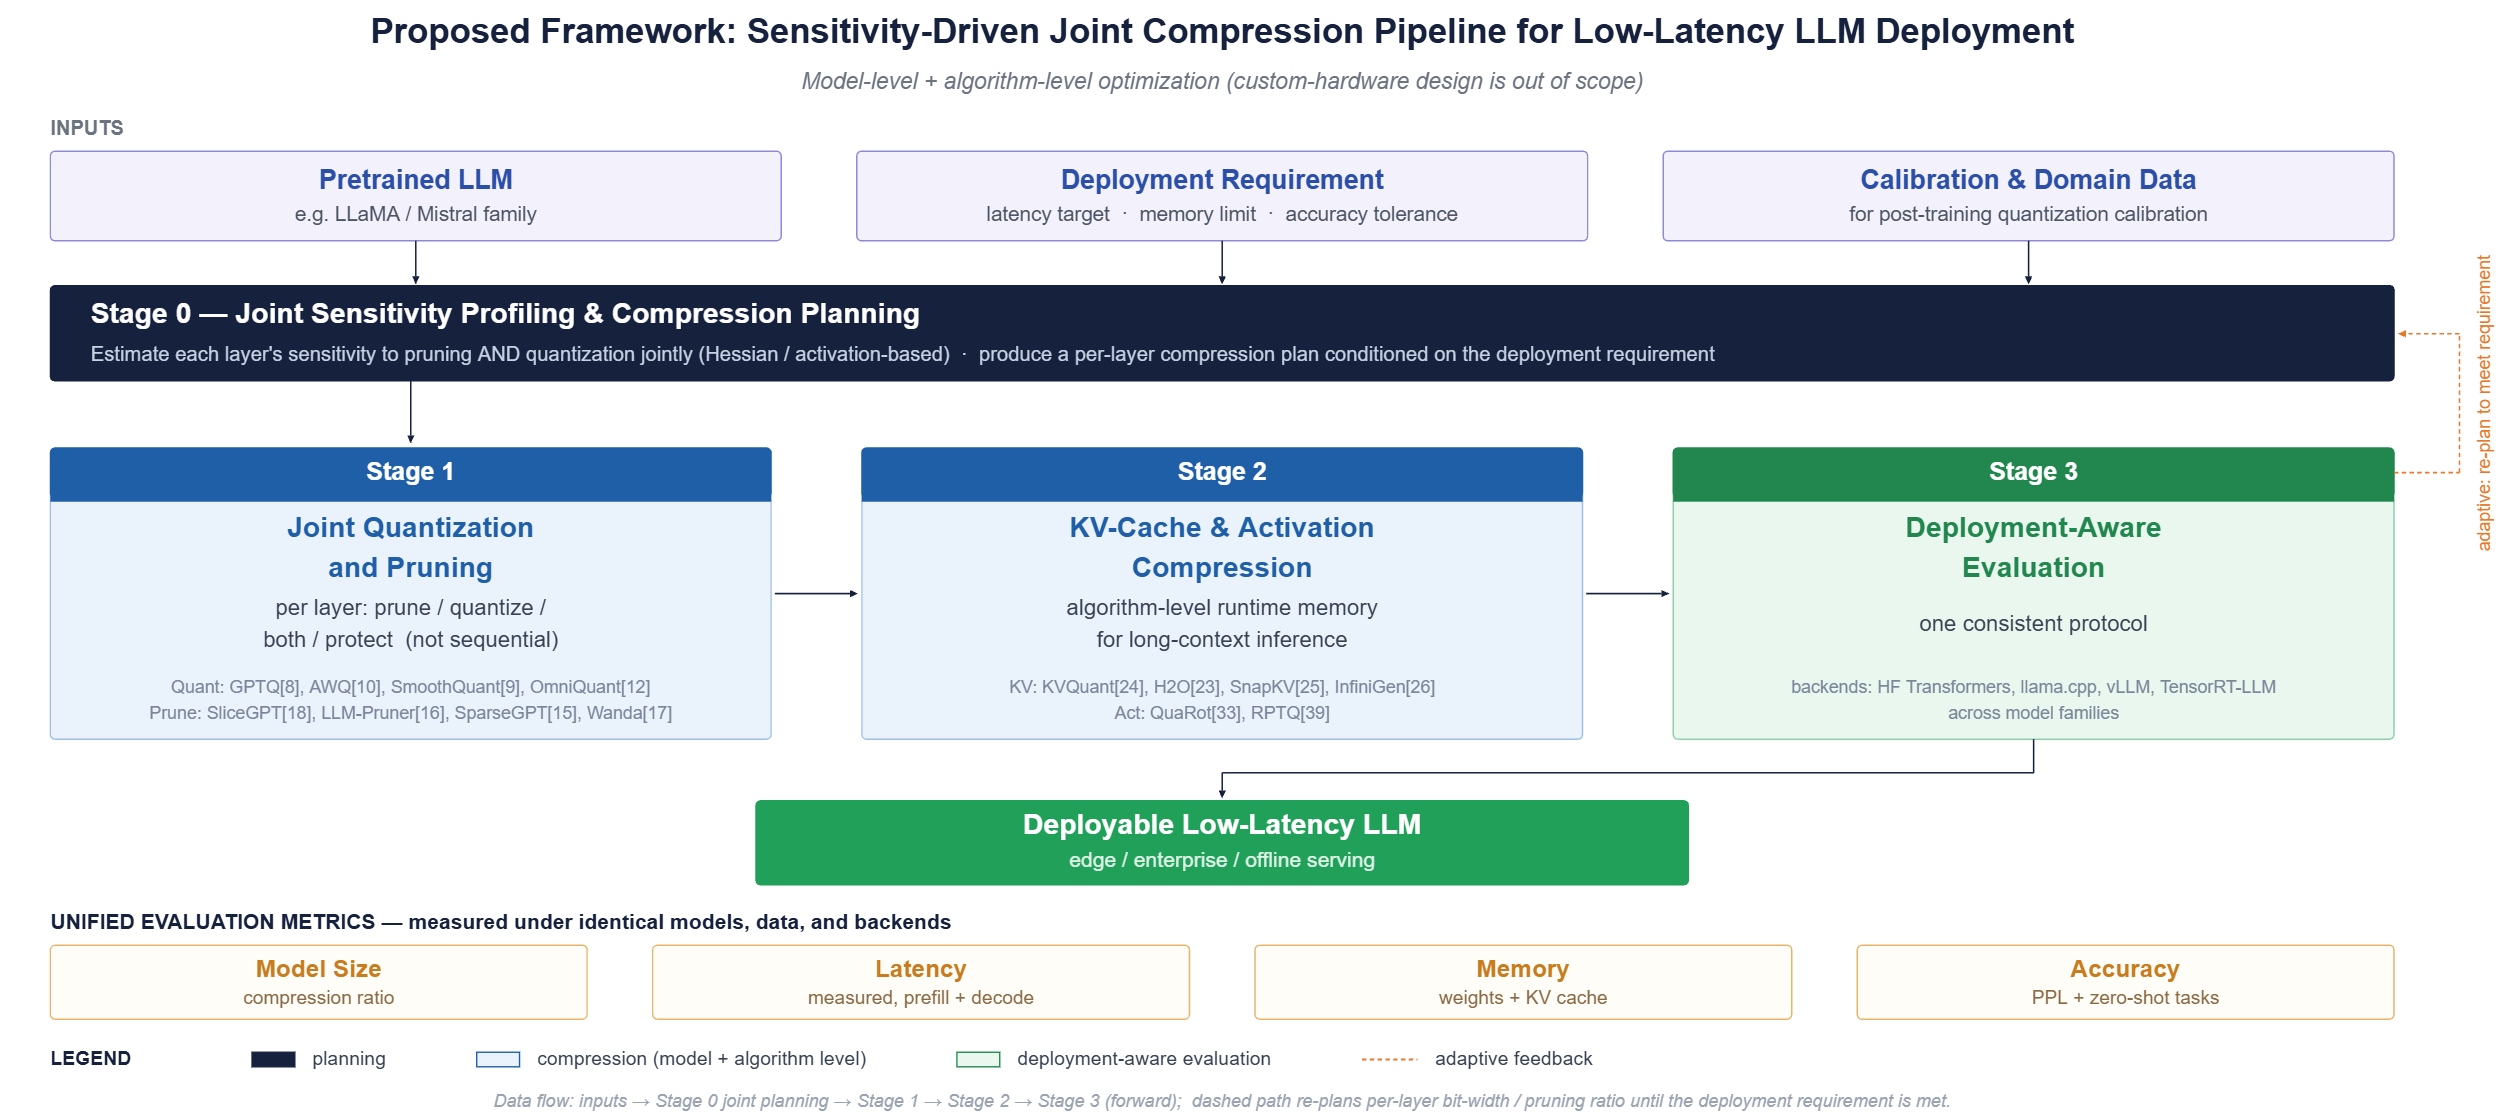
\includegraphics[width=\textwidth]{Figures/lr-fig1-pipeline.png}
\caption{Proposed sensitivity-driven joint compression pipeline. The dashed amber path is the adaptive feedback that re-plans per-layer compression until the deployment requirement is satisfied. Scope is model-level and algorithm-level only.}
\label{fig:lr-pipeline}
\end{figure}

\subsubsection{Key Components and Data Flow}

\begin{itemize}

  \item \textbf{Inputs.} A pretrained LLM; a deployment requirement expressed as a latency target, memory limit, and accuracy tolerance; and calibration/domain data used for post-training quantization calibration and for distillation.

  \item \textbf{Stage 0 --- Joint sensitivity profiling and planning.} Estimates each layer's sensitivity to both pruning and quantization and emits a per-layer plan. This is the only component with a global view and is what makes the pipeline adaptive.

  \item \textbf{Stages 1--4 --- Processing pipeline.} Joint quantization and pruning, distillation-based recovery, KV-cache and activation compression, and deployment-aware evaluation, detailed in the methodology pipeline below.

  \item \textbf{Adaptive feedback.} If evaluation shows the requirement is not met, control returns to Stage 0, which adjusts the per-layer bit-widths, pruning ratios, or KV policy and re-runs the affected stages---turning a one-shot script into a constrained search over the size--latency--memory--accuracy trade-off.

  \item \textbf{Output.} A deployable low-latency model for edge, enterprise, or offline serving, optionally embedded in a retrieval-augmented pipeline.

\end{itemize}

\subsection{Methodology Pipeline}

\subsubsection{Stage 0 --- Joint Sensitivity Profiling and Compression Planning}

The planner characterizes each layer's tolerance to compression using second-order (Hessian-based) and activation-based importance signals---the same signals that underpin the strongest individual methods, e.g. second-order weight quantization \cite{frantar2023gptq}, Hessian-aware mixed-sparsity pruning \cite{shao2024sensitivity}, and activation-aware weight protection \cite{lin2024awq}. Crucially, sensitivity is estimated with respect to \emph{both} pruning and quantization jointly, rather than for one in isolation, so that a layer fragile to one but robust to the other is treated correctly. The output is a per-layer plan---a target bit-width, a pruning ratio, and a ``protect'' flag for the most sensitive layers---chosen to satisfy the deployment requirement. This directly implements the survey's recommendation to estimate how each layer reacts to pruning and low-bit quantization at the same time, instead of running two separate compression steps.

\emph{Techniques that can be used, and how each works (sensitivity signals):}

\begin{itemize}

  \item \textbf{Magnitude scoring} --- ranks weights by absolute value and compresses the smallest first, assuming small weights contribute least; cheapest signal, but blind to how a weight interacts with its inputs.

  \item \textbf{Activation-aware scoring} \cite{lin2024awq,sun2024wanda} --- judges a weight by its magnitude times the size of the input it multiplies. Wanda scores each weight as $|w|\times$ input-feature norm and prunes the lowest per neuron; AWQ scales up the salient channels (those tied to large activations) before rounding so they survive low-bit quantization.

  \item \textbf{First-order / gradient (Taylor) scoring} \cite{ma2023llmpruner} --- estimates the loss increase from removing a weight as roughly $|$weight $\times$ gradient$|$, applied to coupled groups of weights that must be removed together, then recovers with LoRA (LLM-Pruner).

  \item \textbf{Second-order / Hessian scoring} \cite{frantar2023gptq,frantar2023sparsegpt,ling2024slimgpt} --- uses loss curvature: saliency is about $w^2$ over the inverse-Hessian diagonal, and the inverse Hessian also prescribes how to adjust the surviving weights to compensate. GPTQ applies this to rounding, SparseGPT to pruning, SlimGPT to structured pruning.

  \item \textbf{Fisher (squared-gradient) proxy} --- approximates the Hessian with averaged squared gradients, giving curvature-like sensitivity without computing true second derivatives.

  \item \textbf{Representational-change scoring} \cite{yang2024laco,men2024shortgpt} --- scores whole layers by how little they change the hidden state. ShortGPT drops layers whose input and output are nearly identical (low block influence); LaCo merges consecutive near-redundant layers to cut depth.

\end{itemize}

\subsubsection{Stage 1 --- Joint Quantization and Pruning}

Guided by the Stage 0 plan, each layer is compressed by the assigned combination of quantization and pruning in a single coordinated pass. The framework handles the two together rather than one after the other, which is the defining feature distinguishing it from the sequential prune-then-quantize or quantize-then-prune pipelines criticized in the survey.

\textbf{Quantization.} Mixed-precision post-training quantization (PTQ) is the default because it avoids full retraining and is already integrated into common serving libraries; representative operators include one-shot weight-only PTQ \cite{frantar2023gptq}, activation-aware scaling \cite{lin2024awq}, activation-to-weight smoothing \cite{xiao2023smoothquant}, and learnable clipping/transforms \cite{shao2024omniquant}. For extreme low-bit targets the planner may escalate to quantization-aware training \cite{chen2025efficientqat} or post-compression fine-tuning \cite{malinovskii2024pvtuning}.

\begin{itemize}

  \item \textbf{GPTQ} \cite{frantar2023gptq} --- quantizes weights one column at a time and, after each, updates the not-yet-quantized weights via the layer-input inverse Hessian to absorb the rounding error; weight-only 3--4-bit from a small calibration set.

  \item \textbf{AWQ} \cite{lin2024awq} --- identifies the salient weight channels from activation magnitudes and protects them by per-channel scaling before low-bit rounding; weight-only INT3/INT4 with no backpropagation.

  \item \textbf{SpQR} \cite{dettmers2024spqr} --- isolates the few outlier weights with the largest quantization error into a sparse high-precision store and quantizes the dense remainder to 3--4-bit; near-lossless.

  \item \textbf{SmoothQuant} \cite{xiao2023smoothquant} --- divides each activation channel by a scale and multiplies the matching weights by it (identical output), shifting the hard-to-quantize outliers from activations onto weights so both reach INT8 (W8A8).

  \item \textbf{OmniQuant} \cite{shao2024omniquant} --- learns, by gradient descent on each block's reconstruction error, a weight clipping range and an activation-weight smoothing transform; covers W6A6 down to W2A16.

  \item \textbf{QuaRot} \cite{ashkboos2024quarot} --- multiplies weights and activations by Hadamard rotations that cancel across the network, spreading outliers evenly so uniform 4-bit works for weights, activations, and KV cache (W4A4).

  \item \textbf{SpinQuant} \cite{liu2025spinquant} --- uses the same rotation idea but learns the rotation matrices on calibration data instead of using random ones, reducing the residual quantization error.

  \item \textbf{QuIP / QuIP\#} \cite{chee2023quip,tseng2024quipsharp} --- ``incoherence processing'' rotates weights and their Hessian so neither has concentrated large entries, making low-bit rounding provably easier; QuIP\# adds lattice codebooks for vector quantization at or below 4 bits.

  \item \textbf{AQLM} \cite{egiazarian2024aqlm} --- represents each weight group as a sum of vectors drawn from several learned codebooks, jointly optimized to minimize error; reaches 2--3 bits per parameter.

  \item \textbf{QTIP} \cite{tseng2024qtip} --- uses a trellis (stateful sequence) code to obtain a high effective quantization dimension without an exponentially large codebook, combined with incoherence processing.

  \item \textbf{SqueezeLLM} \cite{kim2024squeezellm} --- places non-uniform quantization levels by sensitivity-weighted k-means and splits outlier weights into a sparse high-precision part, targeting the decode memory-bandwidth bottleneck.

  \item \textbf{EfficientQAT} \cite{chen2025efficientqat} --- makes quantization-aware training affordable by first training each block's parameters, then end-to-end training only the quantization scales; 2-bit 70B with a small accuracy drop.

  \item \textbf{PV-Tuning} \cite{malinovskii2024pvtuning} --- recovers accuracy after extreme 1--2-bit compression by going beyond the straight-through estimator, alternately updating the continuous weights and the discrete codeword each maps to.

\end{itemize}

\textbf{Pruning.} Structured pruning is preferred because it yields smaller dense models that accelerate on standard hardware \cite{ma2023llmpruner,ashkboos2024slicegpt,men2024shortgpt}; unstructured or semi-structured pruning \cite{frantar2023sparsegpt,sun2024wanda} is selected only when the target provides sparse-kernel support, since otherwise parameter reduction does not translate into measured speedup. Low-rank factorization \cite{wang2025svdllm} is available as a further dense reduction route.

\begin{itemize}

  \item \textbf{LLM-Pruner} \cite{ma2023llmpruner} --- structural pruning that uses gradient/Taylor importance on coupled groups (heads, channels removed together), then restores accuracy with lightweight LoRA tuning.

  \item \textbf{SliceGPT} \cite{ashkboos2024slicegpt} --- applies a PCA-style orthogonal transform so signal concentrates in the top components, then deletes the least-important rows and columns of the weight matrices, shrinking the hidden dimension into a smaller dense model.

  \item \textbf{ShortGPT} \cite{men2024shortgpt} --- removes whole layers whose input and output hidden states are nearly identical (low block influence).

  \item \textbf{LaCo} \cite{yang2024laco} --- merges consecutive near-redundant layers into one to reduce depth while preserving behaviour.

  \item \textbf{SparseGPT} \cite{frantar2023sparsegpt} --- one-shot unstructured/semi-structured pruning that removes weights and compensates the rest using the layer-input Hessian; reaches 50\%+ sparsity without retraining.

  \item \textbf{Wanda} \cite{sun2024wanda} --- prunes by weight magnitude times input-activation norm, per output neuron, with no retraining or weight update.

  \item \textbf{Sensitivity-aware mixed sparsity} \cite{shao2024sensitivity} --- allocates a different sparsity ratio to each layer from its Hessian sensitivity, pruning robust layers harder and fragile ones less.

  \item \textbf{SVD-LLM} \cite{wang2025svdllm} --- low-rank factorization via truncation-aware SVD that accounts for how the truncation error propagates to the layer output, so the kept components minimize actual output error.

\end{itemize}

\subsubsection{Stage 2 --- Distillation-Based Recovery}

Aggressive joint compression removes capability that must be restored to stay within the accuracy tolerance. Rather than full retraining, the framework applies lightweight recovery: short-horizon knowledge distillation from the original model as teacher, and/or parameter-efficient (LoRA) fine-tuning on the domain corpus. The pruning-then-distillation pattern is well supported, with compact models derived from a larger pretrained model recovering most of the lost quality using a small fraction of the original training data \cite{muralidharan2024minitron}; reverse-KL distillation is used where open-ended generation quality matters \cite{gu2024minillm}. When the target is fixed and small, distillation can be the primary route to a low-latency model, with quantization layered on top.

\begin{itemize}

  \item \textbf{Minitron (prune + distill)} \cite{muralidharan2024minitron} --- prunes a large model in width and depth, then distills the original (teacher) into the pruned student on a small dataset, producing compact models at a fraction of the original training tokens.

  \item \textbf{MiniLLM (reverse-KL distillation)} \cite{gu2024minillm} --- distills with reverse KL divergence instead of forward KL, which stops the student from placing probability on text the teacher would never produce---better suited to open-ended generation.

  \item \textbf{LoRA recovery / LoRAPrune} \cite{ma2023llmpruner,zhang2024loraprune} --- trains small low-rank adapter matrices on the frozen compressed model to recover accuracy cheaply; LoRAPrune additionally uses the LoRA gradients to decide which structures to prune.

  \item \textbf{PV-Tuning} \cite{malinovskii2024pvtuning} --- post-compression fine-tuning for extreme 1--2-bit models that optimizes the discrete codeword assignments rather than relying on straight-through gradients.

  \item \textbf{Distilling Step-by-Step} \cite{hsieh2023distilling} --- extracts natural-language rationales from the teacher and trains the student to predict both the answer and the rationale, so a small model learns the reasoning and needs less data.

\end{itemize}

\subsubsection{Stage 3 --- KV-Cache and Activation Compression}

This stage addresses the runtime, algorithm-level bottleneck that weight compression alone cannot reach. Because the KV cache grows linearly with sequence length and dominates long-context memory and bandwidth, the framework compresses it through low-bit KV quantization \cite{hooper2024kvquant}, heavy-hitter eviction \cite{zhang2023h2o}, per-head selection of important positions \cite{li2024snapkv}, and speculative prefetching in offloading settings \cite{lee2024infinigen}. Activation quantization---which the survey flags as comparatively neglected---is handled with reordering \cite{yuan2023rptq} or rotation-based outlier removal \cite{ashkboos2024quarot}, enabling genuine end-to-end (e.g. W4A4) savings rather than weight-only compression.

\emph{KV cache:}

\begin{itemize}

  \item \textbf{KVQuant} \cite{hooper2024kvquant} --- quantizes the cache to sub-4-bit using per-channel key quantization (keys have channel-aligned outliers), quantizing keys before the rotary position embedding mixes channels, per-token value quantization, and an outlier split---enabling million-token context.

  \item \textbf{H2O} \cite{zhang2023h2o} --- keeps the few ``heavy-hitter'' tokens that carry most of the attention mass, plus recent tokens, and evicts the rest by accumulated attention score; no retraining.

  \item \textbf{SnapKV} \cite{li2024snapkv} --- reads the attention pattern over the end of the prompt to predict which positions each head will keep attending to, and stores only those KV entries per head.

  \item \textbf{InfiniGen} \cite{lee2024infinigen} --- for offloaded caches (KV in CPU memory), speculatively predicts which entries will receive high attention next step and prefetches only those to the GPU, hiding the transfer latency.

\end{itemize}

\emph{Activations:}

\begin{itemize}

  \item \textbf{RPTQ} \cite{yuan2023rptq} --- reorders and clusters activation channels into groups of similar range and quantizes each group with its own scale, pushing activations toward 3-bit.

  \item \textbf{QuaRot / SpinQuant} \cite{ashkboos2024quarot,liu2025spinquant} --- rotate activations (and the KV cache) so outliers are spread out and vanish, enabling clean 4-bit activation quantization (the same rotation methods used in Stage 1).

\end{itemize}

\subsubsection{Stage 4 --- Deployment-Aware Evaluation and Adaptive Re-Planning}

The compressed artifact is evaluated under one consistent protocol across multiple inference backends---Hugging Face Transformers, llama.cpp, vLLM, and TensorRT-LLM---measuring compression ratio, \emph{real} prefill and decode latency, weight and KV memory, energy per token, and accuracy (perplexity plus a zero-shot task suite). Reporting measured latency across backends, rather than parameter reduction in a single setup, is the framework's response to the survey's central methodological concern about inconsistent, single-setup evaluation. If a metric misses the deployment requirement, the adaptive feedback path returns to Stage 0 and the per-layer plan is revised, realizing the adaptive compression the survey calls for.

\begin{itemize}

  \item \textbf{Inference backends} --- measure the same artifact across Hugging Face Transformers, llama.cpp, vLLM, and TensorRT-LLM.

  \item \textbf{Reported metrics} --- compression ratio, measured prefill and decode latency, weight + KV memory, energy per token, accuracy (perplexity + zero-shot suite).

  \item \textbf{Precision-level sweep} --- compare INT8, INT4, and sub-4-bit settings under one identical protocol.

  \item \textbf{Adaptive re-planning} --- feed measured shortfalls back to Stage 0 to adjust bit-width, pruning ratio, or KV policy.

\end{itemize}

\subsection{Methods for Estimating Weight Importance and Allocating Compression}

Before any layer can be compressed, the framework must decide which parts of it matter and how hard each part can be squeezed, because compressing an important weight too aggressively is what makes accuracy fall. This subsection reviews the ways to make that decision. They fall into three broad approaches, plus one technique that recurs across all of them, and are compared in Table~\ref{tab:lr-importance}. The approaches trade how much they cost to compute against how accurate they are, and the strongest pipelines often combine more than one.

\begin{table}[htbp]
\centering
\scriptsize
\caption{Approaches to estimating weight importance and allocating compression: mechanism, representative methods, computational cost, and typical use.}
\label{tab:lr-importance}
\renewcommand{\arraystretch}{1.2}
\begin{tabular}{p{\dimexpr 0.164\linewidth-2\tabcolsep\relax}p{\dimexpr 0.243\linewidth-2\tabcolsep\relax}p{\dimexpr 0.229\linewidth-2\tabcolsep\relax}p{\dimexpr 0.136\linewidth-2\tabcolsep\relax}p{\dimexpr 0.229\linewidth-2\tabcolsep\relax}}
\hline
\textbf{Approach} & \textbf{Mechanism} & \textbf{Representative methods} & \textbf{Computational cost} & \textbf{Best suited to} \\
\hline
Magnitude & Rank weights by size & Baseline & Very low & Quick baselines; mild pruning \\
Activation-aware & Weight size, scaled by its input size & Wanda \cite{sun2024wanda}, AWQ \cite{lin2024awq} & Low & Fast weight-only low-bit plans \\
First-order (gradient) & Estimated error rise if a weight is removed & LLM-Pruner \cite{ma2023llmpruner} & Low--moderate & Structured pruning of coupled blocks \\
Second-order (Hessian) & Error curvature; adjusts the surviving weights & GPTQ \cite{frantar2023gptq}, SparseGPT \cite{frantar2023sparsegpt}, SlimGPT \cite{ling2024slimgpt} & Moderate--high & Accurate low-bit; one-shot pruning \\
Representational change & How much a layer changes its input & ShortGPT \cite{men2024shortgpt}, LaCo \cite{yang2024laco} & Low & Depth pruning / layer dropping \\
Distribution transform & Spread outliers out before quantizing & SmoothQuant \cite{xiao2023smoothquant}, QuaRot \cite{ashkboos2024quarot}, QuIP\# \cite{tseng2024quipsharp} & Moderate & Activation and KV quantization (W4A4) \\
Learned / search & Search or optimize the settings directly & OmniQuant \cite{shao2024omniquant}, AQLM \cite{egiazarian2024aqlm}, DayPQ \cite{xu2026daypq} & High & Extreme compression; adaptive plans \\
\hline
\end{tabular}
\end{table}

\subsubsection{Importance Scoring and Selection}

The most direct approach gives each weight, channel, or layer an importance score, then compresses the low-scoring parts hard and protects the high-scoring ones. The scoring methods range from cheap and rough to expensive and accurate. \emph{Magnitude} scoring ranks weights by size, assuming the largest matter most; it is the cheapest option but ignores how a weight is actually used. \emph{Activation-aware} scoring also looks at the size of the inputs a weight multiplies, so a small weight that handles large inputs is still treated as important---used by Wanda \cite{sun2024wanda} and AWQ \cite{lin2024awq}. \emph{Gradient-based} scoring estimates how much the model's error would rise if a weight were removed; LLM-Pruner \cite{ma2023llmpruner} applies this to groups such as attention heads and channels. \emph{Hessian-based} scoring uses the curvature of the error: near a trained model the slope is flat, so it is the curvature that says how much a small change will hurt---weights in flat directions can be compressed freely, while weights in sharply curved directions must be protected. The same curvature also shows how to adjust the remaining weights to make up for the ones that change, which is the basis of GPTQ \cite{frantar2023gptq}, SparseGPT \cite{frantar2023sparsegpt}, and SlimGPT \cite{ling2024slimgpt}. Because the exact curvature is far too large to compute for billions of weights, it is approximated one layer at a time from a small calibration set, with a cheaper squared-gradient (Fisher) version as a middle ground. Finally, \emph{layer-level} scoring rates whole layers by how much they change the data passing through them: ShortGPT \cite{men2024shortgpt} removes layers that barely change it, and LaCo \cite{yang2024laco} merges layers that do nearly the same work, which is how the model's depth is reduced.

\subsubsection{Distribution Transformation}

A second approach does not score importance at all. Instead, it reshapes the spread of the numbers so that no part is hard to compress. The usual obstacle is a few outlier values, far larger than the rest, that stretch the range which must fit into only a few bits. SmoothQuant \cite{xiao2023smoothquant} moves this difficulty from the activations onto the weights by rescaling, while QuaRot \cite{ashkboos2024quarot}, SpinQuant \cite{liu2025spinquant}, and the related QuIP and QuIP\# \cite{chee2023quip,tseng2024quipsharp} rotate the values in a way that leaves the model's output unchanged but spreads the outliers across many dimensions. Once the outliers are spread out, ordinary low-bit quantization works without having to single anything out, which is what makes compressing weights, activations, and the KV cache together (for example to 4-bit, W4A4) practical.

\subsubsection{Learned and Search-Based Allocation}

A third approach replaces a fixed scoring rule with optimization, letting the method work out the best settings itself. OmniQuant \cite{shao2024omniquant} learns the best rounding ranges and rescaling automatically. Codebook methods fit the set of allowed values to the model's actual weights instead of using evenly spaced levels---AQLM \cite{egiazarian2024aqlm}, QTIP \cite{tseng2024qtip}, and the non-uniform levels in SqueezeLLM \cite{kim2024squeezellm}. Search-based methods choose the configuration for each layer directly: OOPS \cite{survey2026oops} solves an optimization problem for structured pruning, bypass-backpropagation pruning \cite{gao2025bypass} avoids full backpropagation by using a search-based update, and DayPQ \cite{xu2026daypq} picks the pruning and quantization for each layer on the fly. This group is the closest in spirit to the adaptive planner in Stage 0.

\subsubsection{Outlier Detection and Protection}

Running through all three approaches is one recurring technique: find the small set of outlier values and keep only those in high precision, while compressing everything else hard. LLM.int8() \cite{dettmers2022llmint8} picks out outlier activation values by size, SpQR \cite{dettmers2024spqr} isolates the weights that quantize worst, and SqueezeLLM \cite{kim2024squeezellm} splits the weights into a compressed bulk and a small high-precision remainder. Because the same few values tend to drive both pruning and quantization difficulty, finding and protecting them once is a cheap way to recover most of the accuracy that heavy compression would otherwise cost.

In the proposed framework these are not competing winners but a set of options the Stage 0 planner chooses from, depending on how aggressive the target is and how much planning compute is available. A cheap activation-aware score is enough for moderate weight-only quantization; a curvature-based (or Fisher) score is the natural choice when the per-layer plan must stay accurate at very low bit-widths; and a distribution transform is preferred when activations and the KV cache must also be compressed. Outlier protection can be added on top of any of them. TABLE VII: Approaches to estimating weight importance and computational cost, and typical use.

\subsection{Handling Compute, Memory, and Energy Constraints}

Autoregressive inference has two phases with different cost profiles: the prefill phase, which processes the prompt in parallel, is compute-bound, whereas the decode phase, which generates one token at a time, is memory-bandwidth-bound and governs end-to-end latency. The framework therefore treats compute, memory, and energy as explicit constraints, and reducing the per-token cost along these three axes is what yields low-latency inference.

\begin{itemize}

  \item \textbf{Compute.} Compute demand is reduced both structurally and numerically. Structural pruning and low-rank factorization (Stage 1) cut the dimensions of the weight matrices, lowering the number of floating-point operations directly, while layer pruning shortens the sequential depth each token must traverse. Low-bit (INT4/INT8) arithmetic further reduces the cost of each operation on supporting hardware. These reductions are most consequential in the compute-bound prefill phase.

  \item \textbf{Memory.} Memory is managed as two distinct budgets that scale differently. Static weight memory is bounded by weight quantization and structural pruning (Stage 1); the dynamic KV cache, which grows linearly with sequence length and dominates long-context inference, is bounded by KV quantization, eviction, and per-head selection (Stage 3). Because quantization reduces both the bytes stored and the bytes transferred per token, it relieves memory capacity and the decode-phase bandwidth bottleneck at the same time.

  \item \textbf{Energy.} In inference, energy is dominated by data movement rather than arithmetic, since fetching a value from off-chip memory costs substantially more than the operation that consumes it. The same measures that lower memory traffic---lower-precision weights and KV cache, and fewer parameters---therefore reduce energy in approximate proportion to the traffic removed, with reduced-precision arithmetic contributing a further, smaller saving. Energy is consequently handled as a measured budget rather than optimized in isolation.

\end{itemize}

Because Stage 0 plans pruning and quantization together per layer and the feedback loop searches configurations, the framework selects the most aggressive setting that still satisfies the accuracy tolerance; Stage 4 then confirms the resulting compute, memory, and energy savings as measured values on the target backend rather than as theoretical reductions.

\subsection{Evaluation Strategies}

A minimal study on one open model (e.g. a 7B-class LLaMA/Mistral) would mirror the stage order and, in line with the deployment-aware evaluation gap, run the same artifact across several backends:

\begin{itemize}

  \item \textbf{Baseline.} FP16 perplexity (WikiText-2, C4), a zero-shot suite (e.g. PIQA, WinoGrande, ARC), and measured decode latency, memory, and energy on the target.

  \item \textbf{Plan.} Compute joint per-layer pruning/quantization sensitivity; derive a plan for the declared requirement.

  \item \textbf{Compress.} Apply the plan: e.g. structured slicing/pruning \cite{ma2023llmpruner,ashkboos2024slicegpt} plus 4-bit weight PTQ \cite{frantar2023gptq,lin2024awq}, with the most sensitive layers protected.

  \item \textbf{Recover.} Short LoRA/distillation recovery \cite{muralidharan2024minitron}; confirm accuracy returns toward baseline.

  \item \textbf{KV + activations.} Add KV quantization \cite{hooper2024kvquant} and, if needed, activation rotation \cite{ashkboos2024quarot}.

  \item \textbf{Evaluate across backends.} Load the artifact in HF Transformers, llama.cpp, vLLM, and TensorRT-LLM; report the unified metrics and compare. Iterate via the feedback loop until the requirement is met.

\end{itemize}

\section{Conclusion}
\label{sec:lr-conclusion}

This survey reviewed recent quantization and compression techniques for low-latency LLM deployment, covering five thematic directions: quantization-based optimization, pruning and sparsity, hybrid quantization and pruning, knowledge distillation, and KV-cache compression. Approximately fifty papers from major venues were analyzed using a structured thirteen-field taxonomy, and each technique family was compared through dedicated tables addressing methodology, performance, hardware dependency, and deployment considerations.

The comparative analysis showed that quantization is the most prevalent and, in its post-training form, the most readily deployable family, while extreme low-bit and codebook quantization achieves the largest model-size reductions. Pruning provides complementary parameter reduction but delivers reliable speedup mainly in its structured forms, and knowledge distillation reduces cost by producing smaller dense architectures that run well on standard hardware. Hybrid co-designed methods and KV-cache compression report some of the strongest latency and throughput improvements, particularly for long-context inference, indicating that runtime-focused and adaptive optimization is an increasingly important direction.

At the same time, the field faces clear limitations. Reported compression often does not translate into measured latency gains, evaluation is concentrated on high-end GPUs rather than edge devices, extreme quantization still degrades accuracy, unstructured pruning depends on specialized hardware, and energy efficiency is reported inconsistently. The absence of unified benchmarks makes direct comparison across methods difficult.

Continued research in this area remains critical because LLMs are increasingly deployed in latency-sensitive and resource-constrained environments where computational cost, memory bandwidth, and energy consumption are limiting factors. Progress on co-optimized quantization and pruning methods, improved algorithms for extreme low-bit quantization, adaptive compression, and stronger algorithm-level optimization of activations and the KV cache will be essential to make capable LLMs practical across a wide range of real-world deployment settings.
